\section{Anmerkung}
Die App wurde mit NDK entwickelt. NDK ist das Native development Kit von Android.
Mit NDK ruft Java C Methoden auf. Auch die API von ARCore ist eine C-API, generell wird in Android NDK aber mit C++ programmiert und die Schnittstelle in
\begin{verbatim}
  extern "C"{

  }
\end{verbatim}
gekapselt. Deswegen wird im folgenden oft über C oder C++ geredet.

\section{ArCore}
\begin{figure}
  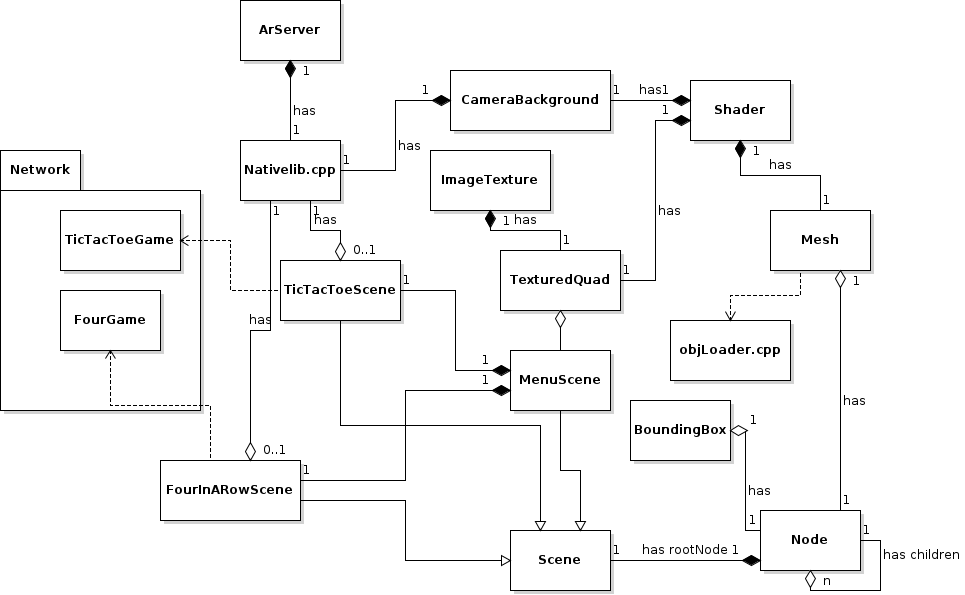
\includegraphics[width=\textwidth]{UML/ArCoreUML.png}
  \caption{Overview of the ArCore/GUI Part of the App}
\end{figure}
\subsection{Entwicklung eines Prototypen}
Am Anfang musste ich die Abhängigkeiten im Buildsystem auflösen, um
ArCore verlinken zu können. Zusätzlich musste ich mich mit dem grundlegenden Lebenszyklus von Apps
auseinander setzten und wegen Android NDK damit beschäftigen, wie man
Parameter von einer Java-Funktion an C übergibt.
Ich habe im nachhinen gemerkt, dass es die Möglichkeit gibt direkt in Android eine
´Native activity´\cite{android_native_activity} zu erstellen die nur C++ nutzt, aber alle OpenGL ES Code-samples von Google\cite{android_ndk_samples_2021},
sowie das AR-Core C Beispiel\cite{ar_core_sdk} nutzen Java mit eingehängten C++ und auch beim erstellen einer
´Native App´ in Android Studio, wird eine Java Activity mit gelinked C++-Code bereitgestellt.
\par
Daraufhin habe ich eine Dummy-
Implementation von ArCore geschrieben, um ArCore zum laufen zu bringen und besser zu verstehen.
Die Dokumentation von Google zu AR-Core war ein wenig kurz gefasst und ich musste dementsprechend immer wieder auf das Beispiel `\verb|hello_ar_c|`, um die Funktionsweise von ArCore zu verstehen.
Lange Zeit zeigte die Kamera kein Bild an, dabei stellte sich heraus das ArCore ein samplerExternalOES anstatt eines einfachen sampler2D benötigt.
\par
Danach merkte ich, dass der Android Emulator nur bedingt OpenGL ES 3.0 supportet\cite{android_emulator_gles3_issue},
deswegen musste ich den Code auf OpenGL ES 2.0 porten, was gerade wegen
Vertex-Array-Objects und eigene Sampler-Objects
umschreiben benötigt hat.
\par
Der Android Emulator hatte einen Bug und somit konnte ArCore App nicht
auf die virtuelle Kamera zugreifen. Das Problem bestand auch bei der Google Beispiel App
``\verb|hello_ar_c|``, aber auch in der Java Version.
\par
Da sich auch heraustellte, dass mein Smartphone ArCore nicht supportet, wurde ich darauf
aufmerksam, dass es eine Liste von supporten Geräten gibt. \cite{ar_core_supported_devices}
\par
Zu dem Zeitpunkt schlug unser Betreuer, Herr Uhlmann, vor auf OpenCV\cite{openCV} zu wechseln, um dementsprechend dem Problem
zu entgehen. Ich schaute mir OpenCV an, aber da die Entwicklung in OpenCV wohl einen sehr viel
größeren Arbeitsaufwand benötigt hätte, entschied ich mich ein ArCore supportetes Gerät zu kaufen.
\par
Auch unser Betreuer, war dementsprechend entgegen kommend und holte sich ein supportes Tablet.

\subsection{Funktionsweise von ArCore}
ArCore\cite{ar_core} ist eine Bibliothek von Google die unter Android ermöglicht AR Applikationen zu entwickeln.
ArCore analysiert dafür den Kamerastream und kann anhand dessen, die Umgebung erkennen.\\
ArCore bietet dafür folgendes:
\\ \\
arCamera: gibt einem Metainformationen über das Kamerabild,sowei eine Projektionsmatrix und Kameramatrix.
\\ \\
arPlane sind Oberflächen die von ArCore erkannt worden sind.(Wird automatisch generiert)
\\ \\
arPoint sind Punkte im reellen 3D Raum die erkannt worden sind.(Wird automatisch generiert)
\\ \\
arAnchor wird vom Entwickler erzeugt, arAnchor erwaret eine Bildposition(zumeist Touchposition), an dieser Bildposition versucht ArCore anhand von eigenen Daten (arPlane,arPoint), den Punkt auf dem geklickt wurde zu erzeugen. Wenn das geklappt hat, wird pro Kameraframe versucht diesen Anchor zu tracken und gibt für diesen Anchor eine Transformationmatrix zurück.


\subsection{Rendering}
\subsubsection{Erste Hilfsklassen}
Für das Rendering habe ich am Anfang ein paar Hilfsklassen gebaut:\\ \\
Shader in Shader.cpp für das lesen von Shadern aus Dateien, compilen und linken.\\ \\
objRenderer in objRenderer.cpp für das Rendern von obj-Files. Später wurde die
Funktionalität in die Mesh Klasse überführt.\\ \\
cameraBackground in cameraBackground.cpp, die das Kamerabild auf einen ScreenQuad sampelt.\\ \\
Aus dem \verb|hello_ar_c| von Google habe ich die objLoader.cpp entnommen, um obj-Dateien
laden zu können.
\subsubsection{Weitere Entwicklung}
Nachdem nun ArCore grundlegend lief habe ich einen Würfel erfolgreich geladen und rendern können.
Nachdem ich dann mit einem Klick auf dem Bildschirm einen
Anchor erzeugen lassen konnte und der Anchor richtig getracked wurde.
Habe ich dann ein simples Szenen System implementiert:
\\ \\
Mesh in Mesh.cpp, dieses lädt eine obj-Datei mithilfe von objLoader.cpp und ermöglicht das rendern dieses Meshes über draw().
\\ \\
Node in Node.cpp enthält
\begin{itemize}
  \item Mesh zum rendern
  \item ModelMatrix in Relation zur Elternnode
  \item Kinder, die auch Nodes sind
\end{itemize}
Scene in Scene.cpp, diese enthält die Root-Node.
Im Konstruktor der Scene werden die Nodes an die Root-Node angehängt oder an andere Nodes die schon angehängt wurden. Beim draw, wird das draw der Root-Node aufgerufen und jede Node ruft widderum
die draw Methode ihrer Childnodes auf und übergibt dabei die eigene Modelmatrix.
\\ \\
Damit wurde das Rendering sehr viel leichter und der Code sehr viel aufgeräumter.

\subsection{Probleme mit ArCore}
Das entwickeln mit ArCore verursachte mehrere Schwierigkeiten, dass größte Problem dabei war
die NDK(C) Version von ArCore. Dabei wurde die objektorientierte API in eine C-API
umgewandelt, was dazu führt, dass wenn in der Javaversion  ein Objekt ein anderes managed,
muss in C immer wieder das Objekt in Aufrufen mitgeschliffen werden.
\\
Hier ein Beispiel, um in der C API, die Modelmatrix von einem getrackten Punkt(anchor) zu bekommen:
\begin{verbatim}
ArPose *pose_;
ArPose_create(arSession, nullptr, &pose_);
ArAnchor_getPose(arSession, anchor, pose_);
ArPose_getMatrix(arSession, pose_, glm::value_ptr(modelMatrix));
ArPose_destroy(pose_);
\end{verbatim}
Siehe \cite{ar_anchor_c} für mehr Details.\\
Wie zu sehen, muss erst eine ArPose erstellt werden, die ArCore erzeugt, dann muss man an diese Pose, die Pose des Anchors binden und kann dann die ModelMatrix bekommen und am Ende muss die Pose wieder gelöscht werden. Dabei muss die arSession immer wieder übergeben werden.
Der gleiche Code in Java:
\begin{verbatim}
modelMatrix = anchor.getPose().toMatrix();
\end{verbatim}
Siehe \cite{ar_anchor_java} für mehr Details.\\
Somit hat es recht lange gedauert, bis ich einen guten Überblick über die C-API
hatte. Am Anfang hatte ich die API direkt in der Nativelib.cpp Datei, die die
Schnittstelle zwischen Java und C++ darstellt und habe diese später in arServer.cpp
migriert, was widerrum die Codekomplexität massiv senkte.

\subsection{Game}
Nachdem ich ArCore und ein gute Szenenabstraktion hatte, habe ich noch eine Hitbox detection geschrieben, diese basiert auf \cite{hitbox_detection}
die mir Herr Uhlmann gab.\\

Danach haben wir unsere beiden Entwicklungsbranches(Netzwerk, ArCore) gemerged, damit konnte ich
dann auf die GameStates zugreifen und dementsprechend für TicTacToe das Feld rendern.
Dabei sind keine größeren Probleme aufgetreten. \\

Da wir jetzt `Vier Gewinnt` implementieren sollten, habe ich die Scene zu einer vererbaren Klasse refactored (in TicTacToeScene.cpp) und daraufhin Vier gewinnt implementiert(FourInARowScene.cpp). \\

Zu guter Schluss habe ich ein Menü eingebaut, dass am Ende des Spiels angibt, ob man
verloren oder gewonnen hat und ein Button, um das Spiel neuzustarten.
Um den Text anzuzeigen habe ich einen TGA Loader geschrieben und musste
erfahren, dass vom Compiler nicht gewährleistet wird, dass structs tightly packed
sind, weshalb die Headerdaten der TGA nicht richtig ausgelesen wurden. Weswegen ich das Problem mehrere Stunden debuggen musste. Mit dem fertigen Menü, war dann auch die App fertig.


\section{Netzerk}
\subsection{Grundlegende Netzwerkfunktion}
Als erstes stellte sich die Frage welche Art der Datenübertragung für TicTacToe und Vier gewinnt am sinnvollsten ist.
Ich musste mich hier zwischen UDP und TCP unterscheiden. Beide haben Vor- und Nachteile, die für Echtzeitspiele zu beachten sind:
\par
Heutige Onlinespiele verwenden häufig UDP, da dieses Protokoll verbindungslos ist.
Das bedeutet bei einer Übertragung wird ein Paket ohne Absicherung verschickt. Der Sender kann dabei nicht wissen ob das Paket
beim Empfänger angekommen ist oder, falls mehrere Pakete gesendet wurden, ob diese in der richtigen Reinheinfolge beim Empfänger
eingetoffen sind.
Bei kurzen Statusmeldungen in Spielen, wie Positionsupdates von Spielern, ist UDP passend, da diese Updates sehr schnell wieder
durch neuere Informationen obsolet werden. Der Client sollte sich also nicht damit beschäftigen alte Pakete zu "retten" sondern
möglichst immer bereit für das neuste Paket sein.
\par
Es gibt aber verschiedene Gründe TCP in Spielen zu verwenden.
Gerade wenn es sich bei den zu übertragenden Daten um wichtige Statusmeldungen handelt, die nur einmalig kommuniziert werden,
ist es wichtig, dass diese beim Empfänger ankommen. Wenn beispielsweise ein Spieler in einem Spiel beitritt, wäre es fatal
wenn diese Information bei einem der Mitspieler nicht ankommt. Die Spielumgebung wäre nicht mehr gleich für alle Teilnehmer
und das Spiel unter Umständen garnicht spielbar. TCP eignet sich sehr gut für solche Statusmeldungen, da es erst eine Verbindung aufbaut.
Solange diese Verbindung existiert, ist garantiert, dass die gesendeten Pakete eintreffen. Auch die richtige Reihenfolge ist garantiert.
\par
Wenn man sich Spiele wie TicTacToe und Vier gewinnt anschaut, bemerkt man schnell das diese Spiele keine großen Mengen von Updates
der Spielumgebung benötigen. Es sind nur wenige, dafür aber kritische Meldungen erforderlich um die Spiele für beide Teilnehmer
synchron zu halten.
\par
Benötigt werden beispielsweise für TicTacToe:
\newline
Statusmeldung wo ein Spieler sein X oder O setzt.
\newline
Statusmeldung ob jemand gewonnen hat und wer.
\newline
Statusmeldung über den Abschluss des Spiels wenn das Spielbrett voll ist und es keinen Sieger gibt.
\newline
Statusmeldung für den Neustart des Spiels.
\par
Alle diese Meldungen sind per TCP besser umzusetzen, da sie in jedem Fall beim Empfänger ankommen müssen. Sonst wäre das Spiel
nicht mehr synchron und ggf. in einem undefinierten Zustand.
\subsection{Implementierung der Grundfunktionen}
Da wir uns für die Entwicklung für Android NDK entschieden haben, setzte ich die Implementierung in C++ um.
Dafür war es notwendig zu verstehen wie C++ mit der normalerweise unter Android verwendeten Programmiersprache Java
zusammen arbeitet.
Das Java Native Interface (JNI) wird benutzt um Objecte zwischen Java und C++ hin und her zu "senden". Diese Übertragungen sind allerdings
zeitaufwendig. Da der visuelle Teil mit ARCore von David auch in C++ implementiert wurde, wollte ich das Netzwerk auch in C++ umsetzen.
\par
Zuerst habe ich Sockets verwendet um Rohdaten empfangen und senden zu können.
In unseren Meetings mit Herrn Uhlmann wurde mir dann vorgeschlagen statt Rohdaten Structs zu verschicken.
Nachdem ich das umgesetzt hatte wurde diese Idee in einem weiteren Meeting erweitert zu Message-Klassen, welche Methoden mitbringen
mit denen die Objekte sich selbst in einen Bytestrom übersetzen und sich aus einem solchen Bytestrom wieder rekonstruieren können.
\subsection{Asnychrones Empfangen}
Als nächstes befasste ich mit dem Asynchronen empfangen der Daten. Da man dauerhaft mit einer Funktion auf eine TCP-Verbindung warten muss
um dann die Nachricht zu verarbeiten, macht es Sinn zumindest das Warten auf neue Verbindungen in einem seperaten Thread zu realisieren.
Dieser Thread ruft dann eine Callbackfunktion auf, die dann mit der Nachricht weiterarbeiten kann.
\subsection{Asynchrones Senden}
Das asynchrone Senden hatte ich mir erst im späteren Verlauf des Projektes vorgenommen. Ich dachte das das Senden nicht sonderlich
zeitaufwendig sein würde und den Spielfluss kaum beeinträchtigen könnte. Damit lag ich falsch. Wenn nämlich ein Fehler beim Senden
auftritt oder das Senden länger braucht als sonst, kann das die ganze App anhalten. Das ist natürlich nicht erstrebenswert.
Also realisierte ich eine Warteschlange in die Nachrichten eingefügt werden. Diese versendet dann der Reihe nach anderer Thread.
Bei einer langsamen Verbindung wird dann nicht die gesamte App verlangsamt.
\subsection{Abstaktion}
In Spielen gibt es im Netzwerk oft eine Hierarchie, welche regelt wer der Host eines Spiels ist und wer nur als Client beitritt.
In unserem Projekt haben wir die Begriffe Master und Slave gewählt.
Der Master hält den einzig wahren Spielzustand. Die Slaves übernehmen diesen und senden dem Master ihre Spielzüge wenn
sie an der Reihe sind. Wenn der Master den Spielzug als valide einstuft werden entsprechende Änderung
am Spielfeld vorgenommen und diese allen Slaves mitgeteilt.
So ändert ein Slave also nie sein eigenes Spielfeld. Nur der Master kann Änderungen für sich und alle Slaves durchführen.
Dadurch wird es viel einfacher die Spielfelder zwischen allen Spielern synchron zu halten.
\subsection{Konkrete Umsetzung für Spiele}
Um für David den Netzwerkcode einfach zugreifbar zu machen, habe ich Subklassen von Master und Slave für das jeweilige Spiel abgeleitet.
Diese können dann genutzt werden um Spielzüge zu machen, ohne dass man sich um die Netzwerkschnittstelle kümmern muss.
Master und Slave sind dann nochmal in einem Game-Objekt zusamengefasst damit David den Code für Master und Slave
einheitlich aufrufen kann.
\subsection{Testen der Netzwerkfunktionen}
Ursprünglich wollte ich den Emulator nutzen um die Kommunikation zwischen zwei Instanzen der App zu testen.
Der Emulator hat allerdings eine eigene Firewall, welche für mich nicht so offensichtlich zu konfigurieren war.
Zusätzlich hatte ich das Problem das mein eigentlicher Arbeitscomputer durch unglückliche Umstände keine Virtualisierung unterstützt.
Dadurch musste ich für die Emulation immer einen seperaten PC verwenden. Das war mir auf Dauer dann zu aufwendig und so entschied ich mich
ein Python-Skript zum schreiben. Damit sollte man das TicTacToe-Spiel in der Kommandozeile gegen einen Spieler mit der App spielen können.
Das Skript kann die Rolle das Masters und des Slaves einnehmen. Damit gelang es dann auch die Netzwerkfunktionen zu testen.

